\subsection{Architecture}

The building blocks of any convolutional neural network are convolution layers,
which, as stated previously, are small-sized learnable filters that are
convolved across an input tensor, and output a visual stimuli under the form of
another tensor, then fed into the next layer.

\begin{figure}[h]
	\center
	\resizebox{480pt}{!}{
		\begin{tikzpicture}
\tikzstyle{connection}=[ultra thick,every node/.style={sloped,allow upside down},draw=\edgecolor,opacity=0.7]
%%%%%%%%%%%%%%%%%%%%%%%%%%%%%%%%%%%%%%%%%%%%%%%%%%%%%%%%%%%%%%%%%%%%%%%%%%%%%%%%%%%%%%%%
%% Draw Layer Blocks
%%%%%%%%%%%%%%%%%%%%%%%%%%%%%%%%%%%%%%%%%%%%%%%%%%%%%%%%%%%%%%%%%%%%%%%%%%%%%%%%%%%%%%%%
% conv1_1,conv1_2
\pic[shift={(0,0,0)}] at (0,0,0) {RightBandedBox={name=cr1,caption=conv1,%
        xlabel={{"64","64"}},ylabel=224,zlabel=224,fill=\ConvColor,bandfill=\ConvReluColor,%
        height=40,width={2,2},depth=40}};
%pool1
\pic[shift={(0,0,0)}] at (cr1-east) {Box={name=p1,%
        fill=\PoolColor,opacity=0.5,height=35,width=1,depth=35}};
%%%%%%%%%%
% conv2_1,conv2_2
\pic[shift={(2,0,0)}] at (p1-east) {RightBandedBox={name=cr2,caption=conv2,%
        xlabel={{"64","64"}},zlabel=112,fill=\ConvColor,bandfill=\ConvReluColor,%
        height=35,width={3,3},depth=35}};
%pool2
\pic[shift={(0,0,0)}] at (cr2-east) {Box={name=p2,%
        fill=\PoolColor,opacity=0.5,height=30,width=1,depth=30}};
%%%%%%%%%%
% conv3_1,conv3_2
\pic[shift={(2,0,0)}] at (p2-east) {RightBandedBox={name=cr3,caption=conv3,%
        xlabel={{"256","256","256"}},zlabel=56,fill=\ConvColor,bandfill=\ConvReluColor,%
        height=30,width={4,4,4},depth=30}};
%pool3
\pic[shift={(0,0,0)}] at (cr3-east) {Box={name=p3,%
        fill=\PoolColor,opacity=0.5,height=23,width=1,depth=23}};
%%%%%%%%%%
% conv4_1,conv4_2,conv4_3
\pic[shift={(1.8,0,0)}] at (p3-east) {RightBandedBox={name=cr4,caption=conv4,%
        xlabel={{"512","512","512"}},zlabel=28,fill=\ConvColor,bandfill=\ConvReluColor,%
        height=23,width={7,7,7},depth=23}};
%pool4
\pic[shift={(0,0,0)}] at (cr4-east) {Box={name=p4,%
        fill=\PoolColor,opacity=0.5,height=15,width=1,depth=15}};
%%%%%%%%%%
% conv5_1,conv5_2,conv5_3
\pic[shift={(1.5,0,0)}] at (p4-east) {RightBandedBox={name=cr5,caption=conv5,%
        xlabel={{"512","512","512"}},zlabel=14,fill=\ConvColor,bandfill=\ConvReluColor,%
        height=15,width={7,7,7},depth=15}};
%pool5
\pic[shift={(0,0,0)}] at (cr5-east) {Box={name=p5,%
        fill=\PoolColor,opacity=0.5,height=10,width=1,depth=10}};
%%%%%%%%%%
% fc6
\pic[shift={(3,0,0)}] at (p5-east) {RightBandedBox={name=fc6,caption=fc6,%
        xlabel={{"1",""}},zlabel=4096,fill=\FcColor,bandfill=\FcReluColor,%
        height=3,width=3,depth=100}};
%%%%%%%%%%
% fc7
\pic[shift={(2,0,0)}] at (fc6-east) {RightBandedBox={name=fc7,caption=fc7,%
        xlabel={{"1","dummy"}},zlabel=4096,fill=\FcColor,bandfill=\FcReluColor,%
        height=3,width=3,depth=100}};
%%%%%%%%%%
% fc8
\pic[shift={(1.5,0,0)}] at (fc7-east) {RightBandedBox={name=fc8,caption=fc8+softmax,%
        xlabel={{"1","dummy"}},fill=\FcColor,bandfill=\FcReluColor,%
        height=3,width=3,depth=25}};

%%%%%%%%%%
% softmax
\pic[shift={(0,0,0)}] at (fc8-east) {Box={name=softmax,%
        xlabel={{"","dummy"}},zlabel=K,opacity=0.8,fill=\SoftmaxColor,%
        height=3,width=1.5,depth=25}};
    
%%%%%%%%%%%%%%%%%%%%%%%%%%%%%%%%%%%%%%%%%%%%%%%%%%%%%%%%%%%%%%%%%%%%%%%%%%%%%%%%%%%%%%%%
%% Draw Arrow Connections
%%%%%%%%%%%%%%%%%%%%%%%%%%%%%%%%%%%%%%%%%%%%%%%%%%%%%%%%%%%%%%%%%%%%%%%%%%%%%%%%%%%%%%%%
\draw [connection]  (p1-east)        -- node {\midarrow} (cr2-west);
\draw [connection]  (p2-east)        -- node {\midarrow} (cr3-west);
\draw [connection]  (p3-east)        -- node {\midarrow} (cr4-west);
\draw [connection]  (p4-east)        -- node {\midarrow} (cr5-west);
\draw [connection]  (p5-east)        -- node {\midarrow} (fc6-west);
\draw [connection]  (fc6-east)       -- node {\midarrow} (fc7-west);
\draw [connection]  (fc7-east)       -- node {\midarrow} (fc8-west);
\draw [connection]  (softmax-east)   -- node {\midarrow} ++(1.5,0,0);
%%%%%%%%%%%%%%%%%%%%%%%%%%%%%%%%%%%%%%%%%%%%%%%%%%%%%%%%%%%%%%%%%%%%%%%%%%%%%%%%%%%%%%%%
%% Draw Dotted Edges 
%%%%%%%%%%%%%%%%%%%%%%%%%%%%%%%%%%%%%%%%%%%%%%%%%%%%%%%%%%%%%%%%%%%%%%%%%%%%%%%%%%%%%%%%
\draw[densely dashed]
    (fc6-west)++(0, 1.5*.2, 1.5*.2) coordinate(a) -- (p5-nearnortheast)
    (fc6-west)++(0,-1.5*.2, 1.5*.2) coordinate(b) -- (p5-nearsoutheast)
    (fc6-west)++(0,-1.5*.2,-1.5*.2) coordinate(c) -- (p5-farsoutheast)
    (fc6-west)++(0, 1.5*.2,-1.5*.2) coordinate(d) -- (p5-farnortheast)
    
    (a)--(b)--(c)--(d)
    ;
%%%%%%%%%%%%%%%%%%%%%%%%%%%%%%%%%%%%%%%%%%%%%%%%%%%%%%%%%%%%%%%%%%%%%%%%%%%%%%%%%%%%%%%%
\end{tikzpicture}

	}
	\caption{The famous VGG-16 architecture.}
	\label{fig:vgg16}
\end{figure}

	\subsubsection{Typical inputs and ouptputs}
In a typical CNN, input and output layers are of a fixed size corresponding to
the problem formulation. The input tensor representing an image can be of any
dimensions, usually with the shape $(H,W,C)$ for $H$ rows corresponding to the
image's height, $W$ columns for its width, and of third axis size $C$ for its
channels (usually 1 for grayscale images and 3 for RGB images). However this
common input shape is not a restriction, and it usually depends on the approach
to the problem: it might be wiser to use square images of cropped grayscale
portraits for face recognition, for instance.\\

\todo{Add tikz image for input and output tensors/vectors}

As for the output, the shape is entirely dependent on the problem and the
desired output of the network. In common image classification implementations,
a one-hot (or multi-hot) encoded vector is usually used as ground truth label,
meaning that the expected output of the network is a vector of size $N$ for $N$
classes.

\begin{wrapfigure}{r}{0.4\textwidth}
	\begin{center}
		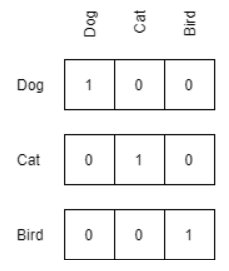
\includegraphics[width=0.24\textwidth]{figure/one_hot.png}
	\end{center}
	\label{fig:onehot}
	\caption{One-hot encoding of 3 classes.}
\end{wrapfigure}


A one-hot encoded vector is a simple representation of the class to which a
given image belongs, where every value is either 0 for the indices corresponding
to the classes which the image does not belong to, or 1 otherwise (see
Figure~\ref{fig:onehot}).\\

Nevertheless, there are many other possible output formats for convolutional
neural networks, such as an other image for the case of auto-encoders or image
segmentation networks. One strong limitation of CNNs is their fixed-sized
input and output layers, which enforces them to be fed with strictly
constrained data. To bypass this constraint, another kind of neural network
must be used, such as recurrent neural netowrks.

	\subsubsection{Layer types}

The pecularities of convolutional neural networks are mainly in the typical
kinds of layers that were not seen in the original perceptron. As it can be seen
on Figure~\ref{fig:vgg16}, convolution layers are usually put in sequence, each
being smaller than the preceiding, as to filter images in a coarse to fine
fashion.\\

The convolution layer owns its naming to the convolution operator, which
consists of summing up the element-wise multiplication between two matrices. In
the case of a CNN, the input layer -- either the input image, or an activation
map produced by a convolution layer -- is convolved with a relatively small
feature detection matrix, called a kernel or filter. The former is learnt by the
network during the training phase, and can be very different from layer to
layer, providing different features detection such as edges, contours, curves,
colors, shapes \emph{etc}\ldots

The kernel is slid over the convolved tensor by $N$ pixels (usually 1), called
the stride, and this dot-product is then appended to the output tensor named
the activation map, or feature map.

The result is a reduced tensor containing the relevant features in the image,
which preserves the spatial relationship between pixels. Having more convolution
layers, and thus more kernels or feature detectors, obviously results in more
features being extracted from the image, and therefore yielding more information
to be used in the final stage of the network, which can make the model more
accurate and more generalized.

Note that convolution layers can also be used in a reversed fashion, to achieve
deconvolution as to upsample an input and generate a higher-resolution tensor.
This practice can be seen in the auto-encoder model, where the goal is to
reconstruct an image from little information of an input.

\todo{Insert convolution picture here}
\begin{figure}[h]
	\center
	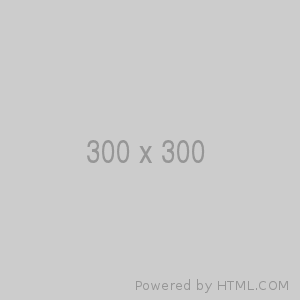
\includegraphics[width=0.4\textwidth]{figure/300x300.png}
	\label{fig:convolution}
	\caption{Convolution of a tensor by a kernel.}
\end{figure}


~\\It is very common to see pooling or sub-sampling layers in-between two
successive convolution layers. The role of the former is to reduce the
dimensionality of the feature map, while preserving the relevant information.


talk about activation layers, relu, softmax
INTRODUCE NON-LINEARITY WITH RELU OR OTHERS
talk about FLCs briefly

talk about additional layers like noise, batch normalization...
